
\section{Solutions to Exercises from Section 2}
\begin{solution}\label{sol:2.1}\ref{ex:2.1}
$$
\begin{aligned}
    &(a) A\times B =\{ (1,a),(1,c),(2,a),(2,c),(3,a),(3,c),(4,a),(4,c) \}\\\\
    &(b) B\times A =\{ (a,1),(c,1),(a,2),(c,2),(a,3),(c,3),(a,4),(c,4) \}\\\\
    &(c) A\times A =A^2= \{ (1,1),(1,2),(1,3),(1,4),(2,1),(2,2),(2,3),\\\\
    &(2,4),(3,1),(3,2),(3,3),(3,4),(4,1),(4,2),(4,3),(4,4) \}\\
    &(d) B\times B = B^2 = \{ (a,a),(a,c), (c,a),(c,c) \}\\\\
    &(e) \varnothing\times B= \{ (a,b):a\in\varnothing,b\in B \}= \varnothing\\\\
    &(f) (A\times B)\times B = \{ (1,a),(1,c),(2,a),(2,c),(3,a),(3,c),(4,a),(4,c) \}\times
    \{ a,c \}=\\
    &\{ ((1,a),a),((1,c),a), ((2,a),a),\\
    &((2,c),a), ((3,a),a),((3,c),a),\\
    &((4,a),a),((4,c),a), ((1,a),c),\\ 
    &((1,c),c),((2,a),c),((2,c),c),\\
    &((3,a),c),((3,c),c),((4,a),c),((4,c),c) \}\\\\
    &(g) A\times (B\times B) = \{ 1,2,3,4 \}\times \{ (a,a),(a,c),(c,a),(c,c) \}=\\
    &\{ (1,(a,a)),(1,(a,c)),(1,(c,a)),(1,(c,c)),\\
    &(2,(a,a)),(2,(a,c)),(2,(c,a)),(2,(c,c))\},\\
    &(3,(a,a)), (3,(a,c)), (3,(c,a)),(3,(c,c)),\\
    &(4,(a,a)),(4,(a,c)),(4,(c,a)),(4,(c,c))\\\\
    &(h) B^3=\{ (a,a,a),(a,a,c),(a,c,a), (a,c,c), (c,a,a),(c,a,c),(c,c,a),(c,c,c) \} = |2^3| = 8
\end{aligned}
$$
This ends Part I of~\ref{ex:2.1}. Now, for part II.\@
$$
\begin{aligned}
    &(a) A\times B= \{ (\pi,0),(\pi,1),(e,0),(e,1),(0,0),(0,1) \}\\\\
    &(b) B\times A= \{ (0,\pi),(1,\pi),(0,e),(1,e),(0,0),(1,0) \}\\\\
    &(c) A^2= \{ (\pi,\pi), (\pi,e),(\pi,0)\\
    &(e,\pi),(e,e),(e,0)\\
    &(0,\pi),(0,e),(0,0) \}\\\\
    &(d) B^2= \{ (0,0),(0,1),(1,0),(1,1) \}\\\\
    &(e) A\times\varnothing=\varnothing\\\\
    &(f) (A\times B)\times B= \{ (\pi,0),(\pi,1),(e,0),(e,1),(0,0),(0,1) \}\times \{ 0,1 \}\\
    &\{  ((\pi,0),0), ((\pi,0),1), ((\pi,1),0), \\
    &((\pi,1),1,), ((e,0),0),((e,0),1),\\
    &((e,1),0),((e,1),1), ((0,0),0),\\
    &((0,0),1), ((0,1),0),((0,1),1)\}\\\\
    &(g) A\times (B\times B)= \{ \pi,e,0 \}\times \{ (0,0),(0,1),(1,0),(1,1) \}\\
    &\{ (\pi,(0,0)),(\pi,(0,1)),(\pi,(1,0)),(\pi,(1,1)),\\
    &(e,(0,0)),(e,(0,1)),(e,(1,0)),(e,(1,1))\\
    &(0,(0,0)),(0,(0,1)),(0,(1,0)),(0,(1,1)) \}\\\\
    &(h) A\times B\times B=\{ (\pi, 0,0),(\pi,0,1),(\pi,1,0),\\
    &(\pi,1,1),(e,0,0),(e,0,1),\\
    &(e,1,0),(e,1,1),(0,0,0),\\
    &(0,0,1),(0,1,0),(0,1,1) \}
\end{aligned}
$$
This concludes part II.\@ Lastly, part III.\@
$$
\begin{aligned}
    &(3)~ \{ x\in\R:x^2=2 \}\times \{ a,c,e \}=\\
    &\{ -\sqrt 2, \sqrt 2 \}\times \{ a,c,e \}=\\
    &\{ (-\sqrt 2, a),(-\sqrt 2, c),(-\sqrt 2, e),\\
    &(\sqrt 2, a),(\sqrt 2,c),(\sqrt 2, e)\}\\\\
    &(4)~ \{ n\in\Z:2<n<5 \}\times \{ n\in\Z:\lvert n \rvert=5 \}=\\
    &\{ 3,4 \}\times \{ -5,5 \}=\{ (3,-5),(3,5),(4,-5),(4,5) \}\\\\
    &(5)~\{ x\in\R:x^2=2 \}\times \{ x\in\R:\lvert x \rvert=2 \}=\\
    &\{ -\sqrt2,\sqrt 2 \}\times \{ -2,2 \}= \{ (-\sqrt 2,-2),(-\sqrt 2,2),(\sqrt 2,-2),(\sqrt 2,2) \}\\\\
    &(6)~\{ x\in\R:x^2=x \}\times \{ x\in\N:x^2=x \}=\\
    &\{ -1,0,1 \}\times \{ 0,1 \}=\\
    &\{ (-1,0),(-1,1),(0,0),(0,1),(1,0),(1,1) \}\\\\
    &(7)~\{ \varnothing \}\times \{ 0,\varnothing \}\times \{ 0,1 \}=\\
    &\{ (\varnothing ,0,0),(\varnothing,\varnothing, 0),( \varnothing ,0,1),( \varnothing , \varnothing, 1) \}\\\\
    &(8)~\{ 0,1 \}{^4}=\{(0,0,0,0),(0,0,0,1),(0,0,1,0),(0,1,0,0),\\
    &(1,0,0,0),(0,0,1,1),(0,1,0,1),(1,0,0,1),\\
    &(0,1,1,0),(1,1,0,0),(1,1,1,0),(1,1,1,1),\\
    &(0,1,1,1),(1,0,1,0), (1,0,1,1),(1,1,0,1)\}.
\end{aligned}
$$


\end{solution}
\begin{solution}\label{sol:2.2}\ref{ex:2.2}
    As in the previous exercise where we sketched out the sets on the $xy$-plane, we will first solve them/explain them and then go on to sketch them.
    $$
    \begin{aligned}
        &(9) \{ 1,2,3 \}\times \{ -1,0,1 \}=\\
        &\{ (1,-1),(1,0),(1,1),\\
        &(2,-1),(2,0),(2,1),\\
        &(3,-1),(3,0),(3,1) \}\\\\
        &(10) \{ -1,0,1 \}\times \{ 1,2,3 \}=\\
        &\{ (-1,1),(-1,2),(-1,3),\\
        & (0,1),(0,2),(0,3),\\
        & (1,1),(1,2),(1,3) \}\\\\
        &(11) [0,1]\times [0,1] \text{ these would be all the paired points in that interval starting from }\\
        &x=0,y=1\\\\
        &(12) [-1,1]\times [1,2] \text{ these would be all the paired points in that interval starting from }\\
        &x=-1,y=1 \text{ and filling the space up to } x=1,y=2\\\\
        &(13) \{ 1,1.5,2 \}\times [1,2] \text{ similarly to the cases above, those will become more obvious when we sketch them out}\\\\
        &(14) [1,2]\times \{ 1,1.5,2 \}, \text{ ditto.}\\\\
        &(15) \{ 1 \}\times [0,1]\\\\
        &(16) [0,1]\times \{ 1 \}\\\\
        &(17) \N\times\Z,\text{ here, we take the natural numbers as our first coordinate and the integers as our second.}\\\\
        &(18) \Z^2,\text{ here we have the whole } xy \text{-plane with whole positive and negative integers.}\\\\
        &(19) [0,1]{^2}\\\\
        &(20) \{ (x,y)\in\R^2:x^2+y^2\le 1 \}\times [0,1].
    \end{aligned}
    $$
    Now, we will show them plotted on the $xy$-plane. 

    % --- FIRST PAGE: Items 9 to 14 ---
\begin{figure}[htbp]
    \centering
    % Item 9
    \begin{subfigure}[b]{0.3\linewidth}
        \centering
        \begin{tikzpicture}[scale=0.6]
            \draw[->] (-0.5,0) -- (3.8,0) node[right] {$x$};
            \draw[->] (0,-1.8) -- (0,1.8) node[above] {$y$};
            \foreach \x in {1,2,3} {
                \foreach \y in {-1,0,1} {
                    \fill[blue] (\x,\y) circle (2.5pt);
                }
            }
        \end{tikzpicture}
        \caption{Item (9)}
    \end{subfigure}\hfill
    % Item 10
    \begin{subfigure}[b]{0.3\linewidth}
        \centering
        \begin{tikzpicture}[scale=0.6]
            \draw[->] (-1.8,0) -- (1.8,0) node[right] {$x$};
            \draw[->] (0,-0.5) -- (0,3.8) node[above] {$y$};
            \foreach \x in {-1,0,1} {
                \foreach \y in {1,2,3} {
                    \fill[blue] (\x,\y) circle (2.5pt);
                }
            }
        \end{tikzpicture}
        \caption{Item (10)}
    \end{subfigure}\hfill
    % Item 11
    \begin{subfigure}[b]{0.3\linewidth}
        \centering
        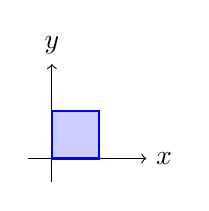
\begin{tikzpicture}[scale=0.6]
            \draw[->] (-0.5,0) -- (2,0) node[right] {$x$};
            \draw[->] (0,-0.5) -- (0,2) node[above] {$y$};
            \fill[blue!20] (0,0) rectangle (1,1);
            \draw[thick, blue] (0,0) rectangle (1,1);
        \end{tikzpicture}
        \caption{Item (11)}
    \end{subfigure}

    \vspace{0.6cm}

    % Item 12
    \begin{subfigure}[b]{0.3\linewidth}
        \centering
        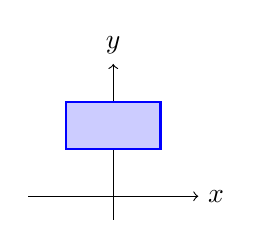
\begin{tikzpicture}[scale=0.6]
            \draw[->] (-1.8,0) -- (1.8,0) node[right] {$x$};
            \draw[->] (0,-0.5) -- (0,2.8) node[above] {$y$};
            \fill[blue!20] (-1,1) rectangle (1,2);
            \draw[thick, blue] (-1,1) rectangle (1,2);
        \end{tikzpicture}
        \caption{Item (12)}
    \end{subfigure}\hfill
    % Item 13
    \begin{subfigure}[b]{0.3\linewidth}
        \centering
        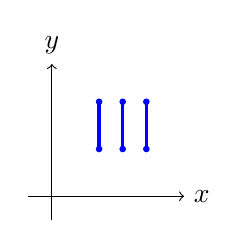
\begin{tikzpicture}[scale=0.6]
            \draw[->] (-0.5,0) -- (2.8,0) node[right] {$x$};
            \draw[->] (0,-0.5) -- (0,2.8) node[above] {$y$};
            \foreach \x in {1,1.5,2} {
                \draw[very thick, blue] (\x,1) -- (\x,2);
                \fill[blue] (\x,1) circle (2pt) (\x,2) circle (2pt);
            }
        \end{tikzpicture}
        \caption{Item (13)}
    \end{subfigure}\hfill
    % Item 14
    \begin{subfigure}[b]{0.3\linewidth}
        \centering
        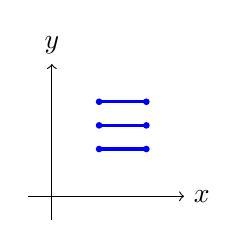
\begin{tikzpicture}[scale=0.6]
            \draw[->] (-0.5,0) -- (2.8,0) node[right] {$x$};
            \draw[->] (0,-0.5) -- (0,2.8) node[above] {$y$};
            \foreach \y in {1,1.5,2} {
                \draw[very thick, blue] (1,\y) -- (2,\y);
                \fill[blue] (1,\y) circle (2pt) (2,\y) circle (2pt);
            }
        \end{tikzpicture}
        \caption{Item (14)}
    \end{subfigure}

    \caption{Plots for Cartesian Products (Items 9--14)}\label{fig:cartesian_1}
\end{figure}

% --- SECOND PAGE: Items 15 to 20 ---
\begin{figure}[htbp]
    \ContinuedFloat%
    \centering
    % Item 15
    \begin{subfigure}[b]{0.3\linewidth}
        \centering
        \begin{tikzpicture}[scale=0.6]
            \draw[->] (-0.5,0) -- (2.2,0) node[right] {$x$};
            \draw[->] (0,-0.5) -- (0,2) node[above] {$y$};
            \draw[very thick, blue] (1,0) -- (1,1);
            \fill[blue] (1,0) circle (2pt) (1,1) circle (2pt);
        \end{tikzpicture}
        \caption{Item (15)}
    \end{subfigure}\hfill
    % Item 16
    \begin{subfigure}[b]{0.3\linewidth}
        \centering
        \begin{tikzpicture}[scale=0.6]
            \draw[->] (-0.5,0) -- (2,0) node[right] {$x$};
            \draw[->] (0,-0.5) -- (0,2) node[above] {$y$};
            \draw[very thick, blue] (0,1) -- (1,1);
            \fill[blue] (0,1) circle (2pt) (1,1) circle (2pt);
        \end{tikzpicture}
        \caption{Item (16)}
    \end{subfigure}\hfill
    % Item 17
    \begin{subfigure}[b]{0.3\linewidth}
        \centering
        \begin{tikzpicture}[scale=0.6]
            \draw[->] (-0.5,0) -- (3.2,0) node[right] {$x$};
            \draw[->] (0,-2.2) -- (0,2.2) node[above] {$y$};
            \foreach \x in {1,2,3} {
                \foreach \y in {-2,-1,0,1,2} {
                    \fill[blue] (\x,\y) circle (2pt);
                }
            }
            \node[blue] at (3.1, 0) {$\dots$};
            \node[blue] at (2, 2.1) {$\vdots$};
            \node[blue] at (2, -2.1) {$\vdots$};
        \end{tikzpicture}
        \caption{Item (17) $\mathbb{N} \times \mathbb{Z}$}
    \end{subfigure}

    \vspace{0.6cm}

    % Item 18
    \begin{subfigure}[b]{0.3\linewidth}
        \centering
        \begin{tikzpicture}[scale=0.6]
            \draw[->] (-2.2,0) -- (2.2,0) node[right] {$x$};
            \draw[->] (0,-2.2) -- (0,2.2) node[above] {$y$};
            \foreach \x in {-2,-1,0,1,2} {
                \foreach \y in {-2,-1,0,1,2} {
                    \fill[blue] (\x,\y) circle (2pt);
                }
            }
            \node[blue] at (2.1, 0) {$\dots$};
            \node[blue] at (-2.1, 0) {$\dots$};
            \node[blue] at (0, 2.1) {$\vdots$};
            \node[blue] at (0, -2.1) {$\vdots$};
        \end{tikzpicture}
        \caption{Item (18) $\mathbb{Z}^2$}
    \end{subfigure}\hfill
    % Item 19
    \begin{subfigure}[b]{0.3\linewidth}
        \centering
        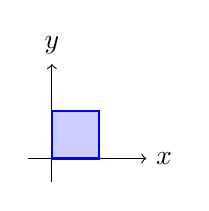
\begin{tikzpicture}[scale=0.6]
            \draw[->] (-0.5,0) -- (2,0) node[right] {$x$};
            \draw[->] (0,-0.5) -- (0,2) node[above] {$y$};
            \fill[blue!20] (0,0) rectangle (1,1);
            \draw[thick, blue] (0,0) rectangle (1,1);
        \end{tikzpicture}
        \caption{Item (19) $[0,1]{^2}$}
    \end{subfigure}\hfill
    % Item 20
    \begin{subfigure}[b]{0.3\linewidth}
        \centering
        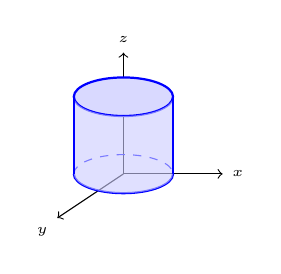
\begin{tikzpicture}[scale=0.7]
            % 3D Axes
            \draw[->] (0,0) -- (1.8,0) node[right] {\tiny $x$};
            \draw[->] (0,0) -- (0,2.2) node[above] {\tiny $z$};
            \draw[->] (0,0) -- (-1.2,-0.8) node[below left] {\tiny $y$};
            
            % Cylinder Body (Solid Disk x [0,1])
            \filldraw[fill=blue!15, draw=blue, thick] (0,1.4) ellipse (0.9cm and 0.35cm);
            \draw[thick, blue] (-0.9,0) arc (180:360:0.9cm and 0.35cm);
            \draw[dashed, blue] (-0.9,0) arc (180:0:0.9cm and 0.35cm);
            \fill[blue!20, opacity=0.6] (-0.9,0) arc (180:360:0.9cm and 0.35cm) -- (0.9,1.4) arc (0:-180:0.9cm and 0.35cm) -- cycle;
            \draw[thick, blue] (-0.9,0) -- (-0.9,1.4);
            \draw[thick, blue] (0.9,0) -- (0.9,1.4);
        \end{tikzpicture}
        \caption{Item (20) Disk $\times [0,1]$}
    \end{subfigure}

    \caption{Plots for Cartesian Products (Items 15--20, Continued)}\label{fig:cartesian_2}
\end{figure}
\end{solution}